\section{Entwurf der Regelungskomponente}
Die Aufgabe der Regelungskomponente besteht darin den Kontroll- und Signalfluss der verschiedenen Versuche zu steuern. Diese Umsetzung erfolgt mit Hilfe eines Zustandautomats, welcher die Trennung der Kontrolllogik und der auszuführenden Aktionen ermöglicht. Des weiteren kann die Applikation bei diesem Ansatz problemlos durch weitere Versuche und Anwendungsfälle erweitert werden. 
Prinzipiell lässt sich der logische Ablauf der Komponente mit einem einfachen Zustandsdiagramm modellieren. Auf der obersten Ebene existiert ein \textit{Standby}-Zustand, der die Inaktivität der Komponente widerspiegelt. Des weiteren enthält diese Ebene Zustände für die verschiedenen Versuche. Diese werden betreten, wenn die Komponente ein Event mit dem entsprechenden Befehl zur Ausführung des Versuchs erhält.
\begin{figure}[h!]
\centering
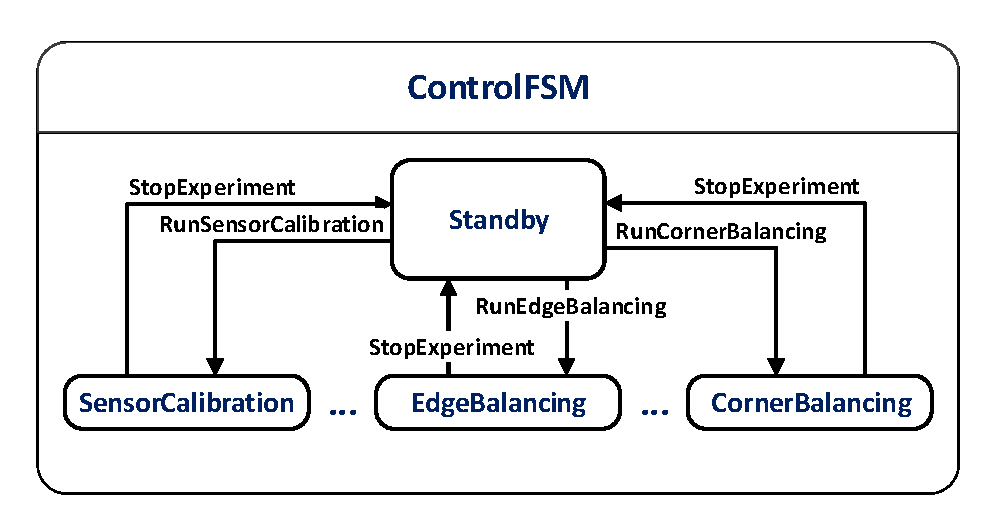
\includegraphics[width=0.7\linewidth]{img/SW_2_ControlComp_SC.pdf}
\caption{Zustandsdiagramm der Kontrol-Komponente, Quelle: eigene Darstellung}
\end{figure}

Ein solches Zustandsdiagramm kann z.B. mit einer objektorientierten Adaption der Methode von Samek [Wie Kapitel14] implementiert werden. Hierbei werden Zustände als Methoden der FSM realisiert, wobei für Oberzustände eigene Klassen entworfen werden, die wiederum Methoden für die jeweiligen Unterzustände besitzen. Die Referenzierung des aktuellen Zustandes erfolgt über einen Funktionenzeiger, der auf die Methode des entsprechenden Zustandes gerichtet ist. 

Als Basis der Typenhierachie dient die abstrakte Klasse \textit{AState}, welche den Zustandstypen als Methodenzeiger definiert, eine Standardimplementierung der \textit{dispatch()}-Methode vorgibt und statische Membervariablen deklariert um die Verarbeitung interner Events zu ermöglichen.
\begin{lstlisting}
class AState
{
protected:
	using StatePtr = bool (AState::*)(CMessage&);
public:
	virtual bool onInitial(CMessage& msg) = 0;
	virtual bool dispatch(CMessage& msg);
	...
protected:
	StatePtr mStatePtr;
	static constexpr StatePtr sInitial = 
			static_cast<StatePtr>(AState::onInitial);
	static CMessage sInternalQueue;
	static UInt32   sQueueSize;
};
\end{lstlisting}
Die Methode \textit{onInitial()} wird verwendet um die FSM und Oberzustände über ein \textit{Init}-Event zu initialisieren. Die \textit{dispatch()}-Methode beschränkt sich auf den Aufruf des aktuellen Zustands.

\begin{lstlisting}
bool AState::dispatch(CMessage& msg)
{
	return *(this->mStatePtr)(msg);
}
\end{lstlisting} 

Die auszuführenden Aktionen, wie z.B. die Berechnung des Regelkreises, werden in der Klasse \textit{CActionHandler} gekapselt. Dadurch erfolgt eine klare Trennung des Kontroll- und Signalflusses. Prinzipiell besitzt \textit{CActionHandler} Methoden, die jeweils beim Betreten und Verlassen der Zustände aufgerufen wird. Zusätzlich kann er um nötige Hilfsmethoden erweitert werden.
\begin{lstlisting}
class CActionHandler
{
public:
	void enterStandby();
	void exitStandby();
	void enterSensorCalibration();
	void exitSensorCalibration();
	...
	void sampleSensorCalibration();
	void sampleEdgeBalancing();
	...
private:
	CThread    mTimerThread;
	CTimerTask mTimerTask;
	
	CHardware         mHardware;
	EdgeBalancingSF   mEdgeBalancingSF;
	ConrnerBalacingSF mCornerBalacingSF;
};
\end{lstlisting}
Für die Zeitgebung wird einer separater Timer-Task \textit{CTimerTask} verwendet, der von \textit{CActionHandler} verwaltet wird. Die Timerklasse kann mittels der Methoden \textit{pause()} und \textit{resume()} pausiert bzw. gestartet werden. Während der Ausführung schläft der Timer für eine konfigurierbare Abtastzeit und erzeugt anschließend über den Proxy ein \textit{TIMERTICK}-Event, welches an die Regelungskomponente weitergeleitet wird.
\begin{lstlisting}
class CTimerTask : public IRunnable
{
public:
	void run() override
	{
		while(true)
		{
			mRunningSem.take(true);
			mRunningSem.give();
			usleep(mPeriod);
			mProxyPtr->timerTick();
		}
	}
	bool pause(bool waitForever){return mRunningSem.take(waitForever);}
	bool resume(){mRunningSem.give();}
	void setPeriod(Int32 period){mPeriod = period;};
	...
private:
	CBinarySemaphore mRunningSem;
	Int32            mPeriod;
	CProxy*          mProxyPtr;
};
\end{lstlisting}
Der Ansatz nach Samek bringt bei diesen Anwendungsfall einen Nachteil mit sich. Für die meisten Versuche genügt eine simple Kontrolllogik, weshalb diese meisten als einfacher Unterzustand realisiert werden. Das hat eine flache Zustandshierarchie zur Folge, die der Anzahl von Versuchen entsprechend breit ist. In der Implementierung resultiert hieraus eine Umfangreiche Klasse \textit{CFSM}, da diese für jeden Unterzustand um eine Methode erweitert wird. Ebenso nimmt der Umfang der Klasse \textit{CActionHandler} mit der Anzahl der Versuche kontinuierlich zu. Dieses Problem kann zwar durch die Aufteilung in mehrere Actionhandler vermieden werden, allerdings wird dadurch die Komplexität von \textit{CFSM} weiter erhöht. Diese Problematik wird dadurch verschärft, dass es sich bei der Zustandsmaschine um den Kern der Anwendung und somit kritischsten Abschnitt der Anwendung handelt. Die zu Grunde liegende Komponentenarchitektur wird zu Projektbeginn erstellt und danach kaum manipuliert. Die dagegen wird während des Projektsverlauf ständig manipuliert, weshalb eine unübersichtliche Implementierung besonders negativ auffällt. Deshalb wird im nächsten Schritte eine alternative Vorgehensweise vorgestellt, die sich die spezielle Struktur des Zustandsdiagrammes zu Nutze macht um eine übersichtliche Implementierung zu schaffen.

Zunächst sei angemerkt, dass es nicht möglich ist direkt zwischen zwei Versuchszuständen zu wechseln. Ein Versuchszustand kann nur aus dem Zustand \textit{Standby} betreten werden. Des weiteren wird nach dem Verlassen eines Versuchszustandes immer in \textit{Standby} gewechselt. Dadurch kann die Kontrolllogik der Zustandsmaschine verallgemeinert werden. Ist der momentane Unterzustand nicht \textit{Standby} und es trifft ein \textit{StopExperiment}-Event ein, so wird der Zustand verlassen und in \textit{Standby} gewechselt. Befindet sich die FSM in \textit{Standby} wird bei Eintreffen eines Events geprüft ob ein Zustandswechsel erfolgen muss. Diese Prüfung kann an die Zustände abgegeben werden. Somit stellt in diesem Fall die Zustandsmaschine lediglich eine Anfrage an alle Versuchszustände ob diese betreten werden möchten.

Die Implementierung der Zustandsmaschine setzt sich folglich aus einem \textit{Standby}-Zustand und einer Liste von Versuchszuständen zusammen. Um eine übersichtliche Codestruktur zu erhalten werden diese als Klassen entworfen, die von der abstrakten Basisklasse \textit{AState} erben.
\begin{lstlisting}
class AState
{
public:
	virtual bool dispatch(CMessage&) = 0;
	virtual bool tryEntry(CMessage&, AState*&) = 0;
	virtual void onEntry() = 0;
	virtual void onExit()  = 0;
private:
	static CMessage sInternalQueue;
	static UInt32   sQueueSize;
};
\end{lstlisting}
Die Methode \textit{dispatch()} dient zur Verteilung von eintreffenden Nachrichten. Mit Hilfe von \textit{tryEntry()} kann die Zustandmaschine prüfen ob der Zustand, in Abhängigkeit des Events, betreten werden möchte. Der folgende Ausschnitt zeigt eine mögliche Implementierung für den Zustand \textit{SensorCalibration}.
\begin{lstlisting}
bool CSensorCalibration::tryEntry(CMessage& msg, AState*& statePtr)
{
	EEvent event = msg.getEvent();
	if(EEvent::RUN_SENSORCALIBRATION == event)
	{
		statePtr = this;
		return true;
	}
	return false;
}
\end{lstlisting}
Das zweite Argument ist eine Zeigerreferenz auf den Zustandsreiger der FSM. Falls ein zustand betreten werden soll überschreibt er die Referenz mit seinem this-Zeiger und gibt \textit{true} zurück um den Konsum des Events zu signalisieren. Die Methoden \textit{onEntry()} und \textit{onExit()} werden zum Betreten bzw. Verlassen des Zustandes verwendet. Um auch die auszuführenden Aktionen zu trennen, wird für jede Zustandsklasse ein Actionhandler implementiert. Diese erben von der Klasse \textit{CActionBase}, die gemeinsame Ressourcen als statische Membervariablen deklariert. Ein Beispiel wären hierfür Instanzen der Klassen \textit{CHardware} oder \textit{CTimerTask}.

Um die Zustandsklassen zu einer Liste zusammenzufassen wird wieder eine lineare Templatehierachie verwendet. Hierfür müss zunächst ein Trägerobjekt \textit{TStateHolder} entworfen werden. 
\begin{lstlisting}
template<class State, class Base>
class TStateHolder : public Base
{
	bool tryEntry(CMessage& msg, AState*& statePtr)
	{
		bool consumed = mState.tryEntry(msg, statePtr);
		if(consumed == false)
		{
			return Base::tryEntry(msg, statePtr);
		}
		return consumed;
	}
private:
	State mState;
};
template<class State>
class TStateHolder<State, CNullType> : public CNullType
{
public:
	bool tryEntry(CMessage& msg, AState*& statePtr)
	{
		return mState.tryEntry(msg, statePtr);
	}
private:
	State mState;
};
\end{lstlisting}
Analog zu \textit{TActionHolder} wird mittels einer Templatespezialisierung unterschieden ob das Ende der Typenliste erreicht ist. Ist dies nicht der Fall wird zunächst geprüft ob der getragene Zustand betreten werden soll. Trifft dies nicht zu wird  die \textit{tryEntry()}-Methode des nächsten Elements in der Hierarchie aufgerufen. Ein Unterschied zu \textit{TActionHolder} ist, dass eine Komposition aus dem Zustandsobjekt verwendet wird. Dadurch werden die Methoden des Zustandes geschützt. Die FSM kann lediglich auf den, über den Zustandszeiger referenzierten, Zustand zugreifen.
Die Implementierung der Zustandsmaschine basiert ebenfalls auf einem Template, welchem die Typenliste der Versuchszustände übergeben wird. Des weiteren erbt die Templateklasse von \textit{AState} um zugriff auf die interne Queue zu erhalten.
\begin{lstlisting}
template<class StateList>
class TFSM : public AState
{
public:
	bool dispatch(CMessage& msg) override;
	bool tryEntry(CMessage& msg, AState*& statePtr) override;
	void onEntry() override;
	void onExit() override;
	bool onStandby(CMessage& msg);
	void handleUnconsumedEvent(CMessage& msg);
private:
	AState*                mStatePtr;
	TLinHierach<StateList> mStateList;
	CAction                mAction;
};
\end{lstlisting}
Neben dem Interface von \textit{AState} besitzt die Klasse zwei weitere Methoden. Wobei die erste den Zustand \textit{Standby} repräsentiert. Die zweite Methode wird genutzt um nicht konsumierte Events, was für gewöhnlich einem Fehlverhalten der FSM entspricht, abfängt. Zunächst wird die \textit{dispatch()}-Methode betrachtet. Hier wird zunächst der aktuelle Unterzustand aufgerufen. Falls das Ereignis nicht konsumiert und es sich um \textit{StopExperiment} handelt, wird der aktuelle Unterzustand verlassen und in \textit{Standby gewechselt}. Zuletzt wird die interne Queue abgearbeitet.
\begin{lstlisting}
template<class StateList>
bool TFSM<StateList>::dispatch(CMessage& msg)
{
	bool consumed = false;
	if(mStatePtr == nullptr)
	{
		consumed = this->onStandby(msg);
	}
	else
	{
		consumed = mStatePtr->dispatch(msg);
	}
	
	if(consumed == false)
	{
		EEvent event = msg.getEvent();
		if(EEvent::StopExperiment == event)
		{
			mStatePtr->onExit();
			mStatePtr = nullptr;
			mAction.entryStandby();
		}
	}
	
	while(squeueSize > 0U)
	{
		CMessage internalMsg(sInternalQueue);
		sQueueSize = 0U;
		consumed = mStatePtr->dispatch(internalMsg);
	}
	return consumed;
}
\end{lstlisting}
Im Zustand \textit{Standby} wird das Ereignis an alle Unterzustände übergeben um zu prüfen, ob diese betreten werden sollen. 
\begin{lstlisting}
template<class StateList>
bool TFSM<StateList>::onStandby(CMessage& msg)
{
	bool consumed = this->tryEntry(msg);
	if(consumed == true)
	{
		mAction.exitStandby();
		mStatePtr->onEntry();
	}
	return consumed;
}
\end{lstlisting}
Die Methode \textit{tryEntry()} stößt lediglich die Abfrage der Unterzustände an.
\begin{lstlisting}
template<class StateList>
bool TFSM<StateList>::tryEntry(CMessage& msg, AState*& statePtr)
{
	return mStateList.tryEntry(mg, statePtr);
}
\end{lstlisting}
Die Vorteile dieses Konzept verdeutlichen sich wieder bei der Anwendung. Für jeden Versuch wird eine Zustandsklasse und Actionhandler entworfen, wodurch eine übersichtliche Projektstruktur entsteht. Um die letztendliche Zustandsmachine zu erhalten wird lediglich \textit{TFSM} mit der gewünschten Liste von Zustandstypen instantiiert.
\begin{lstlisting}
using StateList  = TYPELIST_4(CSensorCalib, CADCCalib, 
                              CEdgeBalance, CCornerBalance);
using ControlFSM = TFSM<StateList>;
ControlFSM myFSM;
\end{lstlisting}
Sollen weitere Zustände hinzugefügt oder entfernt werden muss lediglich die Typdefinition von \textit{StateList} angepasst werden. Um Coderedundanzen zu vermeiden kann für die Unterzustände auch eine Templateklasse entworfen werden, die das Eintrittsereignis und den Actionhandler als Parameter entgegenimmt. Die Unterzustände spezialisieren dann lediglich die Methoden \textit{dispatch()}, \textit{onEntry()} und \textit{onExit()}.
\begin{lstlisting}
/* TSubState.h */
template<const EEvent entryEvent, class Action>
class TSubState : public AState
{
public:
	bool tryEntry(CMessage& msg, AState*& statePtr) override
	{
		if(entryEvent == msg.getEvent())
		{
			statePtr = this;
			return true;
		}
		return false;
	};
	bool dispatch(CMessage& msg) override;
	void onEntry() override;
	void onExit() override;
private:
	Action mAction;
};
\end{lstlisting}

\begin{lstlisting}
/* CADCCalib.cpp */
using CADCCalib = TSubState<EEvent::RunADCCalib, CADCCalibAction>;
template<>
bool CADCCalib::dispatch(CMessage& msg)
{
	EEvent event = msg.getEvent();
	if(EEvent::TIMERTICK == event)
	{
		mAction.sampleADCCalib();
		return true;
	}
	...
	return false;
}
template<>
void CADCCalib::onEntry()
{
	cout << "Entering ADC-Calibration . . . " << endl;
	mAction.resumeTimer();
}
template<>
void CADCCalib::onExit()
{
	cout << "Exiting ADC-Calibration . . . " << endl;
	mAction.pauseTimer();
}
\end{lstlisting}